\newcommand\tab[1][1cm]{\hspace*{#1}}

\section{Introdução}\label{sec}
\tab O presente trabalho tem como finalidade apresentar o resultado da Processo de Engenharia de Requisitos de Software para a Fábrica de Massas do Chef Nery. O empreendimento trata-se de uma micro empresa que fabrica diferentes tipos de massas.\\
\tab O contexto relacionado a necessidade do projeto é principalmente relacionado a necessidade de um melhor gerenciamento de clientes visando então buscar uma melhor forma de gerenciar seus pedidos e divulgar seus produtos.\\
\tab Para isso, é de fundamental importancia utilizar uma metodologia para o levantamento de requisitos e gerenciamento do processo em questão.\\
\tab Com uma análise acerca do contexto foi utilizado uma abordagem ágil composto de atividades do Scaled Agile Framework (SAFe). Com isso, foi possível desenhar o Processo de Engenharia de Requisitos contendo um também um modelo do Processo que será implementado no Trabalho 2.\\

{\large{1.1 Visão Geral do Relatório}}\\ \\
\tab - Introdução: tem como finalidade apresentar um resumo deste documento;\\
\tab - Contexto da Empresa (Chef Nery): fundamenta o contexto da empresa contendo;\\
\tab - Justificativa da Abordagem;\\
\tab - Processo de Engenharia de Requisitos;\\
\tab - Elicitação de Requisitos;\\
\tab - Tópicos de Gerenciamento de Requisitos;\\
\tab - Planejamento do Projeto;\\
\tab - Ferramentas de Gestão de Requisitos;\\
\tab - Considerações Finais;\\
\tab - Referências;\\


\section{Contexto da Empresa (Chef Nery)} % (fold)
\label{sec:nova_sess_o}

\section{Justificativa da Abordagem}
\label{sec:nova_sess_o}

\tab A partir da dećada de 1970, a mudança tecnológica  possibilitou um crescimento exorbitante dos recursos de hardware e permitiram que produtos com tecnologias mais avançadas fossem criadas. Entretanto, as tećnicas utilizadas no desenvolvimento  de software não acompanharam o crescimento dos recursos de hardware, este fenômeno ficou conhecido com a Crise de Software. Neste âmbito, Dijkstra destaca:\\


\tab Não obstante,  ao longo dos anos, notou-se o aumento de metodologias de produção de software com objetivo de aumentar a qualidade e eficiência neste processo. A IEEE define metodologias de desenvolvimento de software como uma abordagem sistemática obtida na etapa de desenvolvimento, no qual, o papel do engenheiro é assegurar que sejam realizadas as melhores escolhas naquele determinado contexto. Vale ressaltar, que estas escolhas têm implicações diretas no sucesso ou fracasso de um projeto.\\

\tab Na etapa de seleção de metodologia foi utilizada o fluxograma proposto pela empresa de consultoria Fortezza Consulting [N]. Apresentado abaixo: \\ 

\tab Desta forma, foram considerada as seguintes perguntas: \\

\begin{enumerate}
	\item \textsl{“Does the scope include software enablement of business processes?”} 
	\item \textsl{“Does the scope include software enablement of business processes?”}
	\item \textsl{“Is the scope lacking in specificity, and unlikely to remain stable?”} 
	\item \textsl{“Is the customer willing and able to offer flexibility on scope?”} 
\end{enumerate}

\tab Com base nas respostas das perguntas acima, foi identificada que a metodologia ágil se adaptaria melhor ao nosso contexto.  

\tab Além disso, uma série de fatores que justificaram o emprego da metodologia ágil, os quais estão descritos abaixo:

\begin{enumerate}
	\item \textsl{Flexibilidade a mudanças;} 
	\item \textsl{Comunicação com o cliente;}
	\item \textsl{Planejamento;} 
	\item \textsl{Equipe de desenvolvedores;}
	\item \textsl{Tamanho do Projeto;}
\end{enumerate}


{
	\large{Flexibilidade a mudanças\\}

	\tab O cliente, dono da fábrica de massas “Chef Nery”, ainda não alcançou uma idéia final concreta sobre o sistema que deseja adquirir. Os requisitos, embora já bem direcionados, permanecem instáveis no que diz respeito à definição de utilidades – ainda não é muito certo tudo o que será essencial ou apenas “bom ter” no projeto. Diante tal contexto, é natural que também o cliente esteja predisposto a flexibilizar o escopo da aplicação, permitindo que se assentem gradualmente as diretrizes definitivas do sistema. \\
	\tab Esta característica é favorável ao uso de metodologias ágeis, que preveem mudanças constantes no escopo e espera flexibilidade dos cliente envolvido [3]. \\
}

{
	\large{Comunicação com o cliente\\}

	\tab O manifesto ágil, criado por  em 1997, propõe uma série de princípios. Dentre eles, destaca-se a interação entre indivíduos como sendo mais relevante que os processos e ferramentas  [3]. Assim,  é necessário que os indivíduos tenham uma comunicação bastante próxima  com o cliente e que as interações com o mesmo possam propiciar mudanças e evolução constantes, possibilitando  a obtenção de requisitos voláteis. \\
	\tab O pequeno tamanho da equipe, que é formada por apenas 4 estudantes de Engenharia de Software e o cliente, somado ao fato de o cliente estar apto e disposto a participar de reuniões e atender as necessidades da equipe de desenvolvimento, possibilita a comunicação próxima da qual as metodologias ágeis se beneficiam. Para tanto, foram adotadas algumas ferramentas de comunicação como o WhatsApp e Hangouts (para situações de impossibilidade de encontros físicos ou necessidade de reuniões emergenciais). \\

}
	
{
	\large{Planejamento\\}

	\tab Em metodologias ágeis, usualmente, as equipes economizam um tempo significativo com o planejamento, visto que as interações que ocorrem junto ao cliente fornecem feedbacks constantes. A título de comparação, em metodologias tradicionais aproximadamente 20 por cento do tempo é gasto na etapas de planejamento e replanejamento [4]. \\
	\tab Não obstante, o cliente em nosso contexto não exige documentação expressiva, pelo contrário valoriza as interações provenientes da metodologia ágil. Desta forma, neste contexto  específico é mais interessante adoção da metodologia ágil,  pois esta  possibilita uma economia de recursos e tempo. \\

}

{
	\large{Equipe de desenvolvedores\\

	\tab A equipe de projetistas e desenvolvedores (que, na verdade, é a mesma equipe) já possui melhor familiaridade com metodologias ágeis, compreendendo relativamente bem suas etapas e rituais. \\
	\tab Somado a isto, há o tamanho diminuto da equipe, que consta 4 integrantes e o cliente, o que possibilita e também facilita uma comunicação intensa e frequente dos integrantes entre si e com o cliente. \\
	\tab Estas características tendem a uma menor dependência de formalidades em documentações e grande dinamicidade na gerência da equipe – ambos fatores que favorecem o uso de metodologias ágeis [5]. \\
}

{
	\large{Tamanho do Projeto\\}

	\tab De acordo com o manifesto ágil, é necessário que os indivíduos tenham uma comunicação bastante próxima com o cliente (BECK et al, 2001). Não obstante, em projetos menores a comunicação é privilegiada visto a maior interação entre os integrantes do projeto. \\
	\tab Além disso, deve-se destacar que em projetos mais complexos, usualmente,  é preferível a utilização de metodologias híbridas ou tradicionais, visto que estas detalham e documentam de forma mais precisa os processos e subprocessos. \\
	\tab Em projetos menores este formalismo é menos relevante, pois existe uma comunicação e um feedback maior entre os envolvidos. \\
}

{
	\large{Scaled Agile Framework(SAFe)\\}

	\tab O SAFe  tem como objetivo sintetizar certos conceitos do corpo do conhecimento e as lições aprendidas de centenas de desenvolvimentos de projetos  dentro de um um único framework, a partir dos seguintes valores:\\

	\begin{enumerate}
		\item \textsl{Alinhamento (Alignment);} 
		\item \textsl{Transparência (Transparency);}
		\item \textsl{Execução do Programa (Program execution);} 
		\item \textsl{Qualidade(Built-in quality);}
	\end{enumerate}

	\tab Assim, este framework escalável tem como objetivo prover práticas providas de metodologias aǵeis, tais como SCRUM e XP em projetos. Além disso, este framework provém artefatos, documentos e atividades e pode ser dividido em três níveis: Portfólio, Programa e Time.\\
	\tab A partir destas características, foi escolhido o SAFe 4.0 ao nosso contexto. Entretanto, foram realizadas algumas adaptações para serem adaptadas ao nosso contexto. Vale ressaltar que o SAFe 4.0 propõe o Value Stream, o qual não foi considerado na elaboração do nosso processo, visto  o tamanho e a simplicidade do projeto \\
}

\section{Processo de Engenharia de Requisitos}
\label{sec:nova_sess_o}


{
	\large{Processo\\}

}

{
	\large{Níveis do Processo\\}

	\tab A seguir serão apresentados os níveis de abstração do processo de Engenharia de Requisitos. Ressalta-se o fato que este processo foi baseado no SAFe 4.0. A seguir serão apresentados estes níveis com maior detalhamento\\ 

}

{
	\large{Nível de Portfólio\\}

	\tab O nível de Portfólio é o nível de abstração mais alto do SAFe. Nesse nível são providos as estruturas necessárias para o desenvolvimento do projeto.  Nele são desenvolvidos: Enables de Épicos; Temas de Investimentos; e os Épicos. \\

}

{
	 \large{Nível de Programa\\}
	 \tab O nível de Programa é o intermédio entre o nível de programa e o do Time. Desta forma, neste nível os times de desenvolvimento e outros recursos são aplicados na tarefa de desenvolvimento do projeto.  Nesta etapa ocorre o refinamento dos Épicos que se transformam em Features e o planejamento do Program Increment (PI).\\
}

{
	\large{Nível de Time\\}

	\tab Este nível se assemelha bastante ao SCRUM,  portanto existem algumas atividades, tais como : Sprint planning, sprint review, sprint retrospective. Nesta etapa, as Features são fragmentadas em Histórias do Usuário. Esta etapa está relacionada com o desenvolvimento dos PI’s. \\
}

{
	\large{Papéis do Processo\\}

	\tab A seguir serão apresentados os papéis adotados para o processo de Engenharia de Requisitos da Fábrica de massas ("Chef Nery"). Ressalta-se o fato que este processo foi baseado no SAFe 4.0. A seguir serão apresentados os papéis do processo.\\

}


{\large{Papéis do Nível de Portfólio\\}}

{
	\large{Gerente de Portfólio\\}

	\tab O Gerente de Portfólio tem como responsabilidade elaborar e comunicar temas estratégicos que implicam nas estratégias da empresa. Ressalta-se também o fato de ser responsável pela elaboração e priorização dos Épicos. \\
	\tab Em nosso contexto, o integrante Eduardo Gomes será o responsável por este papel. \\
}


{
	\large{Arquiteto do Sistema\\}
	\tab O Arquiteto de Sistemas tem a responsabilidade de manter as soluções da empresa de forma holística e iniciativas de desenvolvimento. Além disso, deve fornecer caminhos arquiteturais da empresa que possibilite o suporte aos Enables de Épicos. \\
	\tab Neste contexto, o integrante Miguel Pimentel será o responsável por este papel. \\
}

{\large{Papéis do Nível de Programa\\}}

{
	\large{Gerente do Produto\\}

	\tab O gerente do Produto (Product Manager)  tem como responsabilidade: compreender e entender as necessidades do cliente; validar as soluções desenvolvidas para a necessidade do cliente;  compreender e auxiliar as atividades do nível de Portfólio. Priorizar o fluxo de trabalho do PI; desenvolver Visão; e gerenciar Release. \\
	\tab Em nosso contexto, o papel de gerente do produto será empenhado pelo integrante Miguel Nery. \\
 }


{\large{Papéis do Nível de Programa\\}}

{
	\large{Scrum Master\\}

	\tab O Scrum Master é responsável por asseguram as práticas e princípios do SCRUM e XP. Este papel também deve manter o foco do time, e assim, facilitar o progresso do time. \\
	\tab Em nosso contexto, O Scrum Master será um papel rotativo entre todos os integrantes do time. \\
}

{
	\large{Product Owner\\}

	\tab O Product Owner (PO) é o membro do time responsável pela definição das histórias e priorização do Backlog tanto como simplificar as prioridades do programa. \\
	\tab O PO também pode realizar algumas tarefas conhecidas, tais como: desenvolvimento e participação no PI planning; definir metas da sprint; definir prioridades  a partcir do backlog; execução do programa; manter o programa; trabalhar em harmonia com o Product Manager; participar do planejamento e validação da sprint. \\
	\tab Em nosso contexto, PO será empenhado por Pedro Nery (Dono da fábrica de massas “Chef Nery”). \\
}

{
	\large{Desenvolvedores (Time)\\}

	\tab O time também conhecido como Equipe de Desenvolvedores está relacionado com o terceiro nível de abstração. Além disso, é responsável pela pela entrega de uma versão usável de cada incremento provido de um PI. \\
	\tab Em nosso contexto, todos os integrantes da equipe realizaram o papel de desenvolvedores. \\

}

{
	\large{Artefatos do Processo \\}

	\tab A seguir serão apresentados os artefatos oriundos do processo de obtenção de Requisitos da Fábrica de massas ("Chef Nery"). Ressalta-se o fato que este processo foi baseado no SAFe 4.0. A seguir serão apresentados os artefatos como uma breve descrição destes. \\

}

{\large{Artefatos em Nível de Portfólio \\}}

{
	\large{Temas de Investimento \\}

	\tab Temas estratégico é artefato responsável por todas as questões de negócio do projeto. Este artefato é relacionado com o nível de abstração Portfólio. \\
}


{
	\large{Backlog de  Épicos \\}

	\tab O Backlog de Épicos é um artefato que engloba os épicos que foram levantados juntos a cliente e serão produzidos. Vale ressaltar que eles possuem um priorização. \\
}

{\large{Artefatos em Nível de Programa \\}}

{
	\large{Visão \\}

	\tab A artefato de visão descreve uma noção das soluções a serem desenvolvidas, refletindo as necessidades do cliente e stakeholders, como também as features e soluções propostas a estas necessidades. \\
}


{
	\large{Backlog de Features \\}

	\tab Apresenta o conjunto de features que serão implementadas para o sistema, estas devem estar pontuadas de acordo com a sua dificuldade técnica. Pode-se utilizar ferramentas como o planning poker para a avaliação da dificuldade técnica das features levantadas. \\
}

{
	\large{Roadmap \\}

	\tab Apresenta os entregáveis próximos a partir de uma linha do tempo, em outras palavras, apresenta as features organizadas de acordo com a priorização definida previamente. \\
}

{
	\large{Especificação Suplementar\\}

	\tab Este artefato apresenta todas as definições necessárias do negócio não incluídas na definição de Requisitos funcionais, no caso, Backlog de Features e Backlog do Time. \\
}

{\large{Artefatos em Nível de Time \\}}

{
	\large{Backlog do Time \\}

	\tab Representa um conjunto de histórias priorizada de acordo com os interesses do cliente. Elas consistem da fragmentação e refinamento das features definidas no nível do programa. Além disso, o Backlog do time também pode ser entendido como o conjunto de todas as coisas que o time deve fazer. \\
}

{
	\large{Sprint Backlog\\}

	\tab Consiste em todas as histórias de usuário que devem ser desenvolvidas durante uma sprint. Vale ressaltar que estas histórias são oriundas do Backlog do Time. \\
}

{

	\large{Atividades do Processo \\}

	\tab As atividades  estão dispostas a seguir de acordo com o quadro apresentado abaixo. Não obstante, cada atividade se encontra no subtópico referente ao seu nível de abstração. \\
	\tab No quadro abaixo, o identificador foi criado para identificar a atividade de acordo com o seu nível de abstração. Desta forma, os identificadores estão representados da seguinte maneira: \\

	\begin{itemize}
		\item Atividades que começarem com as iniciais PO, referem-se ao nível de abstração Portfólio e o número da atividade neste nível. Exemplo: PO01 (Atividade 1 do nível de abstração Portfólio);\\
		\item Atividades que começarem com as iniciais PR, referem-se ao nível de abstração Programa e o número da atividade neste nível. Exemplo: PR01(Atividade 1 do nível de abstração Programa);\\
		\item Atividades que começarem com as iniciais T, referem-se ao nível de abstração Time e o número da atividade neste nível. Exemplo: T03(Atividade 3 do nível de abstração Time); \\
	\end{itemize}

	\tab Além disso, para atividades que não são necessárias entradas ou possuem não apresentam nenhuma saída será identificado pela sigla N/A (Não se aplica).\\

	\onecolumn
		\begin{usecase}
    		\addtitle{Processo}{ }

    		\addfield
    			{Nome:}{Nome da atividade coeso com a atividade que deve ser realizada}
			\addfield
    			{Identificador:}{Identifica a atividade conforme foi descrito anteriormente}
    		\addfield
    			{Descrição:}{Breve descrição da atividade}
    		\addfield
    			{Entrada:}{Indica qual dos artefatos serão utilizados na realização desta atividade}
    		\addfield
    			{Saída:}{Indica os artefatos que foram elaborados ao término desta atividade}
			\addfield
    			{Responsável:}{Indica qual dois papéis é responsável pela execução  desta atividade}

		\end{usecase}
	\onecolumn

}

{
	\large{Atividades do Nível de Portfólio}

	\onecolumn
		\begin{usecase}
    		\addtitle{Atividade:}{Compreender o contexto e os objetivos do cliente}

    		\addfield
    			{Nome:}{Compreender o contexto e os objetivos do cliente}
			\addfield
    			{Identificador:}{PO01}
    		\addfield
    			{Descrição:}{Compreender quais são as necessidades do cliente  a partir do contexto que ele está inserido}
    		\addfield
    			{Entrada:}{N/A}
    		\addfield
    			{Saída:}{Temas de Investimento}
			\addfield
    			{Responsável:}{Gerente de Portfólio}

		\end{usecase}
	\onecolumn

	\onecolumn
		\begin{usecase}
    		\addtitle{Atividade:}{Definir Épicos}

    		\addfield
    			{Nome:}{Definir Épicos}
			\addfield
    			{Identificador:}{PO02}
    		\addfield
    			{Descrição:}{Definir os Épicos de acordo com as necessidade e contexto do cliente}
    		\addfield
    			{Entrada:}{Temas de Investimento}
    		\addfield
    			{Saída:}{Épicos}
			\addfield
    			{Responsável:}{Gerente de Portfólio}

		\end{usecase}
	\onecolumn

	\onecolumn
		\begin{usecase}
    		\addtitle{Atividade:}{Definir Enables para os Épicos}

    		\addfield
    			{Nome:}{Definir Enables para os Épicos}
			\addfield
    			{Identificador:}{PO03}
    		\addfield
    			{Descrição:}{Definir quais serão os enables para os épicos previamente definidos}
    		\addfield
    			{Entrada:}{Épicos}
    		\addfield
    			{Saída:}{Enables de Épicos}
			\addfield
    			{Responsável:}{Gerente de Portfólio e Arquiteto do Sistema}

		\end{usecase}
	\onecolumn

	\onecolumn
		\begin{usecase}
    		\addtitle{Atividade:}{Priorizar Épicos }

    		\addfield
    			{Nome:}{Priorizar Épicos}
			\addfield
    			{Identificador:}{PO04}
    		\addfield
    			{Descrição:}{Definir quais épicos devem possuir maior prioridade sobre os outros}
    		\addfield
    			{Entrada:}{Enables de Épicos e Épicos}
    		\addfield
    			{Saída:}{Backlog de Épicos}
			\addfield
    			{Responsável:}{Gerente de Portfólio }

		\end{usecase}
	\onecolumn

	\onecolumn
		\begin{usecase}
    		\addtitle{Atividade:}{Validar Épicos}

    		\addfield
    			{Nome:}{Validar Épicos}
			\addfield
    			{Identificador:}{PO05}
    		\addfield
    			{Descrição:}{Validar junto ao cliente se os Épicos atendem suas necessidade}
    		\addfield
    			{Entrada:}{Backlog de Épicos}
    		\addfield
    			{Saída:}{N/A}
			\addfield
    			{Responsável:}{Product Owner e  Gerente de Produto}

		\end{usecase}
	\onecolumn


}

{
	\large{Atividades do Programa\\}

	\onecolumn
		\begin{usecase}
    		\addtitle{Atividade:}{Elaborar Visão}

    		\addfield
    			{Nome:}{Elaborar Visão}
			\addfield
    			{Identificador:}{PR01}
    		\addfield
    			{Descrição:}{Desenvolver o artefato de visão }
    		\addfield
    			{Entrada:}{Backlog de Épicos e Temas de Investimento}
    		\addfield
    			{Saída:}{Visão}
			\addfield
    			{Responsável:}{Arquiteto do Sistema e Gerente do Produto}

		\end{usecase}
	\onecolumn

	\onecolumn
		\begin{usecase}
    		\addtitle{Atividade:}{Gerenciar Requisitos}

    		\addfield
    			{Nome:}{Gerenciar Requisitos}
			\addfield
    			{Identificador:}{PR02}
    		\addfield
    			{Descrição:}{Identificar, avaliar e acordar modificações nos requisitos}
    		\addfield
    			{Entrada:}{Temas de Investimento, Épicos }
    		\addfield
    			{Saída:}{Atualização dos requisitos}
			\addfield
    			{Responsável:}{Gerente do Produto}

		\end{usecase}
	\onecolumn

	\onecolumn
		\begin{usecase}
    		\addtitle{Atividade:}{Definir Features}

    		\addfield
    			{Nome:}{Definir Features}
			\addfield
    			{Identificador:}{PR03}
    		\addfield
    			{Descrição:}{Refinar os Épicos com o objetivo de obter features}
    		\addfield
    			{Entrada:}{N/A}
    		\addfield
    			{Saída:}{Features}
			\addfield
    			{Responsável:}{PO, Arquiteto de Sistema e Gerente do Produto }

		\end{usecase}
	\onecolumn

	\onecolumn
		\begin{usecase}
    		\addtitle{Atividade:}{Elaborar Requisitos Não-Funcionais}

    		\addfield
    			{Nome:}{Elaborar Requisitos Não-Funcionais}
			\addfield
    			{Identificador:}{PR04}
    		\addfield
    			{Descrição:}{Definir características e necessidades do sistema que não seja funcionalidades}
    		\addfield
    			{Entrada:}{N/A}
    		\addfield
    			{Saída:}{Especificação Suplementar}
			\addfield
    			{Responsável:}{Gerente do Produto, Arquiteto do Sistema e PO}

		\end{usecase}
	\onecolumn

	\onecolumn
		\begin{usecase}
    		\addtitle{Atividade:}{Definir Enables para Features}

    		\addfield
    			{Nome:}{Definir Enables para Features}
			\addfield
    			{Identificador:}{PR05}
    		\addfield
    			{Descrição:}{Definir recursos que permitam a execução das features}
    		\addfield
    			{Entrada:}{Features}
    		\addfield
    			{Saída:}{Enables para Features}
			\addfield
    			{Responsável:}{Arquiteto do Sistema e Gerente do Produto}

		\end{usecase}
	\onecolumn

	\onecolumn
		\begin{usecase}
    		\addtitle{Atividade:}{Priorizar Features}

    		\addfield
    			{Nome:}{Priorizar Features}
			\addfield
    			{Identificador:}{PR06}
    		\addfield
    			{Descrição:}{Definir quais features devem possuir maior prioridade sobre os outros}
    		\addfield
    			{Entrada:}{Features}
    		\addfield
    			{Saída:}{Backlog de Features}
			\addfield
    			{Responsável:}{Gerente do Produto e PO}

		\end{usecase}
	\onecolumn

	\onecolumn
		\begin{usecase}
    		\addtitle{Atividade:}{Elaborar Roadmap}

    		\addfield
    			{Nome:}{Elaborar Roadmap}
			\addfield
    			{Identificador:}{PR07}
    		\addfield
    			{Descrição:}{Elaborar o artefato Roadmap}
    		\addfield
    			{Entrada:}{Visão e Backlog das Features}
    		\addfield
    			{Saída:}{Roadmap}
			\addfield
    			{Responsável:}{Arquiteto do Sistema e Gerente do Produto}

		\end{usecase}
	\onecolumn

	\onecolumn
		\begin{usecase}
    		\addtitle{Atividade:}{Validar Features}

    		\addfield
    			{Nome:}{Validar Features}
			\addfield
    			{Identificador:}{PR08}
    		\addfield
    			{Descrição:}{Validar junto ao cliente se as features atendem suas necessidades}
    		\addfield
    			{Entrada:}{Backlog de Features}
    		\addfield
    			{Saída:}{Backlog Atualizado}
			\addfield
    			{Responsável:}{Product Owner e  Gerente do Produto}

		\end{usecase}
	\onecolumn

	\onecolumn
		\begin{usecase}
    		\addtitle{Atividade:}{Elaborar PI(Program Increment)}

    		\addfield
    			{Nome:}{Elaborar PI(Program Increment)}
			\addfield
    			{Identificador:}{PR09}
    		\addfield
    			{Descrição:}{Definir quais serão os incrementos do produto de acordo com as necessidades do cliente}
    		\addfield
    			{Entrada:}{Visão e Backlog de Features}
    		\addfield
    			{Saída:}{Incremento de Software}
			\addfield
    			{Responsável:}{Gerente do Produto, Arquiteto do Sistema, PO, Scrum Master}

		\end{usecase}
	\onecolumn\onecolumn
		\begin{usecase}
    		\addtitle{Atividade:}{}

    		\addfield
    			{Nome:}{}
			\addfield
    			{Identificador:}{}
    		\addfield
    			{Descrição:}{}
    		\addfield
    			{Entrada:}{}
    		\addfield
    			{Saída:}{}
			\addfield
    			{Responsável:}{}

		\end{usecase}
	\onecolumn

	\onecolumn
		\begin{usecase}
    		\addtitle{Atividade:}{}

    		\addfield
    			{Nome:}{}
			\addfield
    			{Identificador:}{}
    		\addfield
    			{Descrição:}{}
    		\addfield
    			{Entrada:}{}
    		\addfield
    			{Saída:}{}
			\addfield
    			{Responsável:}{}

		\end{usecase}
	\onecolumn

	\onecolumn
		\begin{usecase}
    		\addtitle{Atividade:}{}

    		\addfield
    			{Nome:}{}
			\addfield
    			{Identificador:}{}
    		\addfield
    			{Descrição:}{}
    		\addfield
    			{Entrada:}{}
    		\addfield
    			{Saída:}{}
			\addfield
    			{Responsável:}{}

		\end{usecase}
	\onecolumn


}

	



\section{Elicitação de Requisitos}
\label{sec:nova_sess_o}

\tab Uma Elicitação de requisitos tem por característica achar o que realmente o usuário precisa para uma futura implementação de um software, é um processo que define o que o software deve ter como funcionalidade. Elicitar também pode ser descrito como descobrir ou obter informação sobre algo. O sucesso de um sistema de informação depende da qualidade da definição dos requisitos [10]. A isso se deve a grande importância de fazer um bom levantamento de requisitos.\\
\tab Diversos projetos de software possuem a característica de terem falhado por problemas de Elicitação de Requisitos [8] [9]. Pode ser entendido que muitas vezes, os requisitos são mal interpretados ou incompletos. Com uma elicitação mal feita estariam comprometidos tanto a documentação quanto a especificação dos requisitos, provocando a inviabilidade de todo processo de Engenharia de Requisitos.\\
\tab O processo de Engenharia de requisitos é a primeira etapa dentro de todo o processo de Engenharia de Requisitos [11]. Nela, a principal preocupação é em como levantar os reais requisitos do sistema. Para isso, existem diversas maneiras de levantar requisitos. \\

{\large{5.1. Técnicas de Elicitação de Requisitos}}\\ \\
\tab Foram estabelecidos critérios para a seleção das técnicas de elicitação de requisitos usadas. Estes foram:\\ \\
\tab - Disponibilidade da Equipe;\\
\tab - Disponibilidade do Cliente;\\
\tab - Compatibilidade das Técnicas com a abordagem.\\ \\
\tab A partir desses critérios serão/foram utilizadas as seguintes técnicas:\\

{\large{5.1.1. Observação}}\\ \\
\tab Essa técnica tem por característica possibilitar um contato pessoal estreito do pesquisador com o fenômeno pesquisado [12], no caso do presente projeto, um dos integrantes tem ligação parentesca com o cliente, isso facilita muito tanto a comunicação quanto o entendimento do trabalho para todo o grupo.\\

{\large{5.1.2. Entrevista}\\ \\
\tab Essa é uma técnica que tem como base o engenheiro ou analista discutir o sistema com diferentes usuários, a partir disso elabora um entendimento dos requisitos [12]. No caso foi feita uma entrevista aberta, em que houve uma conversa para determinar o que o cliente necessita a partir de seus problemas.\\

{\large{5.1.3. Protótipo}}\\ \\
\tab É um sistema sem funcionalidades inteligentes. O protótipo cria uma interface para o cliente validar o software que será implementado.\\

{\large{5.1.4. Workshop}}\\ \\
\tab É uma técnica tem um objetivo pré determinado onde cada indivíduo tem direito a fala e são discutidos os requisitos de acordo com esse objetivo. Em um Workshop há um indivíduo que é responsável por conduzir a reunião e gerar discussões entre os envolvidos.\\

\label{sec:nova_sess_o}

\section{Planejamento do Projeto}
\label{sec:nova_sess_o}

\section{Ferramentas de Gestão de Requisitos}
\label{sec}
\tab Foram realizadas pesquisas comparativas entre as ferramentas para gerir os requisitos, podendo elas serem versões Web ou ainda em versão de Desktop. Foram escolhidas então: Jira, Innoslate e Rally Dev.\\

{\large{8.1 Critérios}}\\

\tab Para esta análise, foram listadas 5 características julgadas importantes para a gestão de requisitos para o projeto, referentes à Usabilidade, Rastreabilidade, Gestão de Mudanças, Flexibilidade e Licença.\\
\tab \textbf{Usabilidade:} Analisa se a usabilidade da ferramenta é de fato intuitiva ou não, o que pode vir a trazer contratempos para a equipe.\\
\tab \textbf{Licença:} Analisa a licença da ferramenta, caso seja grátis, paga, se possui isenção para projetos educativos, etc.\\
\tab \textbf{Rastreabilidade:} Analisa se é possível rastrear de forma eficaz a ferramenta.\\
\tab \textbf{Gestão de Mudanças:} Analisa quais são as funcionalidades que ajudam na gestão de mudanças, análise de impacto, e escopo.\\
\tab \textbf{Flexibilidade:} Analisa a flexibilidade de personalização da ferramenta ao contexto do projeto.\\

{\large{8.2 Pontuação}}\\

\tab Para conseguir escolher com exatidão, foi atribuído uma pontuação a tais características com o intuito de esclarecer numericamente qual a ferramenta que nos auxiliaria. A pontuação foi ponderada de 0 à 5 sendo mais próximo de 5 muito pertinente às necessidades do projeto, e mais próximo de 0 muito divergente do fim das reais necessidades do projeto.\\

{\large{8.3 Resultados}}\\

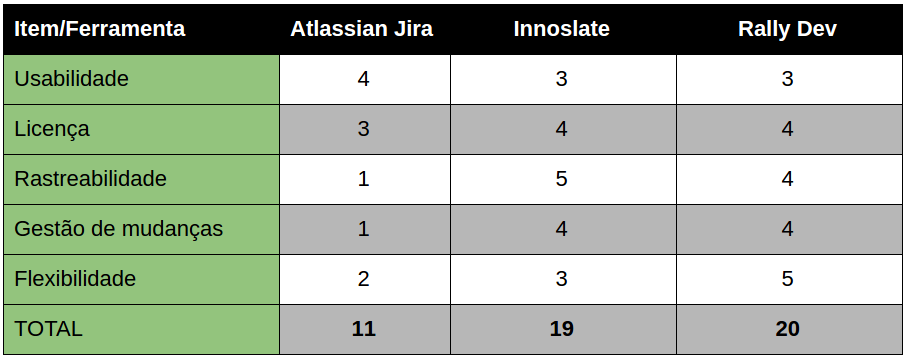
\includegraphics[width=1\textwidth]{conteudo/resultados}\\

{\large{8.4 Descrição das notas atribuídas}}\\

\textbf{Usabilidade:}\\
	\tab Atlassian Jira: Interface bonita; Nomes bem intuitivos; Plugins gráficos interessantes.\\
	\tab Innoslate: Interface satisfatória; \\
	\tab RallyDev: Interface satisfatória; Ícones intuitivos;\\

\textbf{Licença:}\\
	\tab Atlassian Jira: Gratuito por 30 dias;\\
	\tab Innoslate: Versão grátis, com restrições;\\
	\tab RallyDev: Versão grátis, com restrições;\\

\textbf{Rastreabilidade:}\\
	\tab Atlassian Jira : Hierarquia pouco intuitiva; não existe ferramenta visual para controlar importância de requisitos em relação aos demais.\\
	\tab Innoslate: Rastreabilidade bastante intuitiva; Geração automática de índice de qualidade de requisitos e numeração na criação de entidade.\\
	\tab RallyDev: Hierarquia com fácil localização; Opção de linkar requisitos filhos;\\

\textbf{Gestão de mudanças:}\\
	\tab Atlassian Jira: Não aparenta ter algum feedback de mudanças do próprio autor ou de outros autores;\\
	\tab Innoslate: Controle de versão eficaz; Notificações com últimas alterações com autor e data;\\
	\tab RallyDev: Controle de versão eficaz;\\

\textbf{Flexibilidade:}
	\tab Atlassian Jira: Não apresenta ter opção de personalização;\\
	\tab Innoslate: Opções de fixar e desafixar abas importantes para o projeto;\\
	\tab RallyDev: Totalmente flexivel para modificações relevantes para o projeto com inúmeras possibilidades de plugins.\\

{\large{8.5 Escolha da ferramenta}}\\

\tab Após uma profunda análise em cada uma das ferramentas estudadas, foi decidido que o Rally Dev será utilizada para o gerenciamento de requisitos. Suas características de personalização e controle de versão foram fundamentais para a criação do próprio modelo de rastreabilidade do projeto.  \\


\section{Considerações Finais}
\label{sec:nova_sess_o}

\section{Referências}
\label{sec:nova_sess_o}




\onecolumn
\begin{usecase}
    \addtitle{Caso de Uso 1}{Exemplo de caso de uso}

    \addfield{Resumo:}{\lipsum[1]}

    \addfield{Ator Primario:}{Manolo}

    \addfield{Pré-condições:}{Aplicativo instalado}
\end{usecase}
\onecolumn

\onecolumn
\begin{figure}[h]
  \begin{center}
    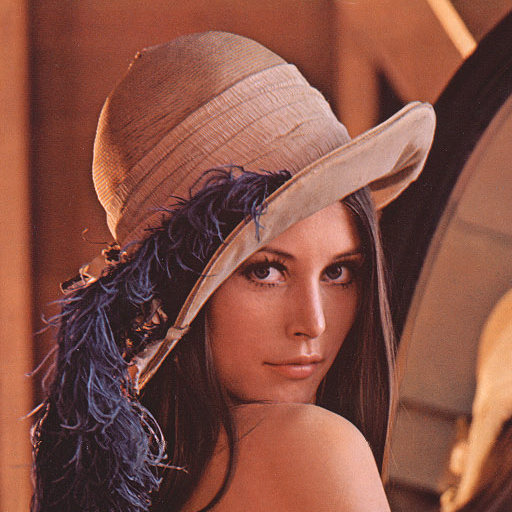
\includegraphics[width=0.8\textwidth]{conteudo/lena}
    \caption{Clássica Lena}
  \end{center}
\end{figure}
\onecolumn

\onecolumn

\begin{longtable}{  c  L{1.5cm}  C{1.2cm}  R{2.5cm}  p{2cm}  m{3.5cm}  }
\caption{Entidade: Motorista}\\
\toprule
Nome & Tipo & Tamanho  & Restrições de Domínio & Regra de Derivação & Observações \\ \midrule
\rowcolor[gray]{0.9}
CNH & Integer & 11 & - & - & Campo que armazena o número da CNH \\
Nome & Char & 30 & - & - & Campo que armazena o nome do motorista \\
\rowcolor[gray]{0.9}
CPF & Char & 20 & Somente números & - & Campo que armazena o número do CPF \\
RG & Char & 20 & Somente números & - & Campo que armazena o número de RG \\ \bottomrule
\end{longtable}

\onecolumn

